\documentclass[11pt,aspectratio=43]{beamer} \usepackage[utf8]{inputenc}
\usepackage{amsmath, amsfonts, amssymb, amsthm}
\usepackage[T1]{fontenc}
\usepackage{lmodern}
\usepackage{xcolor}
\usepackage[nodisplayskipstretch]{setspace}
\usepackage{booktabs}
\usepackage{multirow}
\usepackage{graphicx}
\usepackage{tikz}
% \usetikzlibrary{decorations}
\usetikzlibrary{decorations.pathreplacing}
\usepackage{ulem}
\usepackage{hyperref}
\usepackage{booktabs}
\usepackage{babel}
\usepackage{makecell}
\usepackage[para,online,flushleft]{threeparttable}
\usepackage{pdfpages}
\usepackage{tcolorbox}
\usepackage{bm}
\usepackage{appendixnumberbeamer}
\usepackage{natbib}
\usepackage{caption}
\captionsetup[figure]{labelformat=empty}% redefines the caption setup of the figures environment in the beamer class.
\usetheme[compress]{Boadilla}
\usecolortheme{default}
\useoutertheme{miniframes}
\usefonttheme[onlymath]{serif}

\newcommand{\jump}[2]{\hyperlink{#1}{\beamerbutton{#2}}}
\newcommand{\orange}[1]{\textcolor{orange}{#1}}
\newcommand{\red}[1]{\textcolor{red}{#1}}

\setbeamertemplate{itemize item}{\raisebox{0.1em}{\scalebox{0.7}{$\blacksquare$}}}
\setbeamertemplate{itemize subitem}[circle]
\setbeamertemplate{itemize subsubitem}{--}
\setbeamercolor{itemize item}{fg=black}
\setbeamercolor{itemize subitem}{fg=black}
\setbeamercolor{itemize subsubitem}{fg=black}
\setbeamercolor{item projected}{bg=darkgray,fg=white}
\definecolor{blue}{rgb}{0.2, 0.2, 0.7}
\setbeamercolor{alerted text}{fg=blue}
\setbeamertemplate{enumerate items}[circle]



\setbeamertemplate{headline}{}

%==========================================
\let\olditemize=\itemize
\let\endolditemize=\enditemize
\renewenvironment{itemize}{\olditemize \itemsep1em}{\endolditemize}
\let\oldenumerate=\enumerate
\let\endoldenumerate=\endenumerate
\renewenvironment{enumerate}{\oldenumerate \itemsep1em}{ \endoldenumerate}

\DeclareMathOperator*{\argmax}{\arg\!\max}
\DeclareMathOperator*{\E}{\mathbb{E}}
\DeclareMathOperator*{\var}{\rm Var}
\DeclareMathOperator*{\cov}{\rm Cov}

\theoremstyle{definition}
\newtheorem{assume}{Assumption}
\newtheorem{lem}{Lemma}
\newtheorem{proposition}{Proposition}
\newtheorem{thm}{Theorem}
\newtheorem{corol}{Corollary}

\begin{document}
    \title[Lecture 7]{Lecture 7 \\ Representative Firm}
    \author[Hui-Jun Chen]{Hui-Jun Chen}
    \institute[OSU]{The Ohio State University}
    % \date{\today}
    \date{\today}
    \setbeamertemplate{navigation symbols}{}
    \setstretch{1.2}

%-------------------------------------------------------
{
%	\usebackgroundtemplate{\includegraphics[width=1\paperwidth]{../EveningSky_cropped_edit43_bright.jpg}}
    \begin{frame}
% \vspace{3em}
        \centering
%		{\footnotesize 	ECON 4002 Intermediate Macroeconomic Theory}
        \maketitle
% \vspace{-1.5em}
% \centering
% \includegraphics[width=0.55\linewidth]{Pictures/houses.jpeg}


    \end{frame}
}

% -------------------------------------------
\setbeamertemplate{headline}
{
\setbeamercolor{section in head/foot}{fg=black, bg=white}
\vskip1em \tiny \insertsectionnavigationhorizontal{1\paperwidth}{\hspace{0.50\paperwidth}}{}
}
%------------------------------------------

\begin{frame}{Overview: Lecture 4 - 7}
\label{slide:Overview__Lecture_4_7}

\begin{center}
Provide \alert{micro-foundation} for the \alert{macro implication} (\alert{Lucas critique})
\end{center}

\begin{itemize}
    \item \textbf{Representative Consumer}:
    \begin{itemize}
        \item Lecture 4: \alert{preference}, \alert{constraints}
        \item Lecture 5: \alert{optimization}, \alert{application}
        \item Lecture 6: Numerical Examples
    \end{itemize}
    \item \textbf{Representative Firm}:
    \begin{itemize}
        \item Lecture 7: \alert{production}, \alert{optimization}, \alert{application}
    \end{itemize}
\end{itemize}
\end{frame}

\section{Technology}
\label{sec:Technology}

\begin{frame}{Production Function}
\label{slide:Production_Function}
    \textbf{Production function} describes the technology possibility for \alert{converting inputs into outputs}.

    Representative firm produces output $ Y $ with production function
    %
    \begin{equation}
    \label{eq:production}
         Y = z F( K, N^{d} )
    \end{equation}
    %
    \begin{itemize}
        \item $ Y $: output (consumption goods)
        \item $ z $: \alert{total factor productivity (TFP)} (productivity for the economy)
        \item $ K $: capital (fixed for now, $ \because $ 1-period model)
        \item $ N^{d} $: labor demand (chose by firm, \alert{d} represents demand)
    \end{itemize}
\end{frame}

\begin{frame}{Properties of Production Function: Marginal Product}
\label{slide:Properties_of_Production_Function__Marginal_Product}
\begin{itemize}
    \item  \textbf{Marginal product}: how much $ Y \uparrow $ by one unit of $ K \uparrow  $ or $ N^{d} \uparrow $.
    \begin{itemize}
        \item \textbf{Marginal product of capital} (MPK): $z D_{K}F( K, N^{d} )$
        \item \textbf{Marginal product of labor} (MPN): $z D_{N}F( K, N^{d} )$
    \end{itemize}
    \item Marginal product is \alert{positive} and \alert{diminishing}:
    \begin{itemize}
        \item \textbf{Positive MP}: $ Y \uparrow  $ if either $ K\uparrow  $ or $ N^{d} \uparrow  $
        \begin{itemize}
            \item more inputs result in more output
        \end{itemize}
        \item \textbf{Diminishing MP}: MPK $ \downarrow  $ as $ K \uparrow  $; MPN $ \downarrow  $ as $ N^{d}  \uparrow  $
        \begin{itemize}
            \item the \alert{rate/speed} of output increasing is decreasing
        \end{itemize}
    \end{itemize}
    \item \textbf{Increasing marginal cross-products}:
    \begin{itemize}
        \item e.g. MPK $ \uparrow  $ as $ N \uparrow  $; MPN $ \uparrow  $ as $ K \uparrow  $
    \end{itemize}
\end{itemize}
\end{frame}

\begin{frame}{Properties of Production Function: Return to Scale}
\label{slide:Properties_of_Production_Function__Return_to_Scale}
    \begin{itemize}
        \item \textbf{Return to scale}: how $ Y $ will change when both $ K $ and $ N $ increase
        \item \textbf{Constant return to scale} (CRS): $ x z F( K, N^{d} ) = z F( xK, xN^{d} ) $
        \begin{itemize}
            \item small firms are \alert{as efficient as} large firms
        \end{itemize}
        \item \textbf{Increasing return to scale} (IRS): $ x z F( K, N^{d} ) > z F( xK, xN^{d} ) $
        \begin{itemize}
            \item small firms are \alert{less efficient than} large firms
        \end{itemize}
        \item \textbf{Decreasing return to scale} (DRS): $ x z F( K, N^{d} ) < z F( xK, xN^{d} ) $
        \begin{itemize}
            \item small firms are \alert{more efficient than} large firms
        \end{itemize}
    \end{itemize}
\end{frame}

\begin{frame}{Example: Cobb-Douglas Production Function}
\label{slide:Example__Cobb_Douglas_Production_Function}
    \begin{itemize}
        \item \textbf{Cobb-Douglas}: $ z F( K, N ) = z K^{\alpha} N^{1-\alpha}$, $ \alpha $ is the share of capital contribution to output
        \item \textbf{Positive MPK \& MPN}:
        \begin{itemize}
            \item MPK $ = D_{K}z F( K, N ) = z \alpha K^{\alpha-1} N^{1-\alpha} = z \alpha \left( \frac{K}{N} \right)^{\alpha-1} > 0$
            \item MPN $ = D_{N}z F( K, N ) = z ( 1-\alpha ) K^{\alpha} N^{-\alpha} = z ( 1-\alpha ) \left( \frac{K}{N} \right)^{\alpha} > 0$
        \end{itemize}
        \item \textbf{Diminishing MP}:
        \begin{itemize}
            \item For $ K $, $ D_{K} \left( z \alpha K^{\alpha-1} N^{1-\alpha} \right) = z \alpha \red{( \alpha - 1 )} K^{\alpha - 2} N^{1-\alpha} < 0$
            \item For $ N $, $ D_{N} ( z ( 1-\alpha ) K^{\alpha} N^{-\alpha} ) = z ( 1-\alpha ) \red{( -\alpha )} K^{\alpha} N^{-\alpha-1} < 0$
        \end{itemize}
        \item \textbf{Increasing marginal cross-product}:
        \begin{itemize}
            \item For MPK, $ D_{N} ( z \alpha K^{\alpha-1} N^{1-\alpha} ) = z \alpha ( 1-\alpha ) K^{\alpha-1}N^{-\alpha} > 0$
            \item For MPN, $ D_{K} ( z ( 1-\alpha ) K^{\alpha} N^{-\alpha}  )  = z ( 1-\alpha ) \alpha K^{\alpha-1} N^{-\alpha} > 0$
        \end{itemize}
    \end{itemize}
\end{frame}

\begin{frame}{Example: Cobb-Douglas and Return to Scale}
\label{slide:Example__Cobb_Douglas_and_Return_to_Scale}

Let's assume that Cobb-Douglas production is $ z F( K, N ) = z K^{\alpha} N^{\beta} $

So if both inputs are increasing by twice, then

%
\begin{align*}
    zF( 2K, 2N )
        & = z ( 2K )^{\alpha} ( 2N )^{\beta} = 2^{\alpha} \times 2^{\beta} z K^{\alpha} N^{\beta}
    \\
        & = 2^{\alpha+\beta} z K^{\alpha} N^{\beta} = 2^{\alpha+\beta} Y
\end{align*}
%
\begin{enumerate}
    \item If $ \alpha+\beta = 1 $, then $ zF( 2K, 2N ) = 2Y $, constant return to scale
    \item If $ \alpha+\beta < 1 $, then $ zF( 2K, 2N ) = 2^{\alpha+\beta}Y < 2Y $, decreasing return to scale
    \item If $ \alpha+\beta > 1 $, then $ zF( 2K, 2N ) = 2^{\alpha+\beta}Y > 2Y $, increasing return to scale
\end{enumerate}
<++>




\end{frame}



\begin{frame}{Visualization}
\label{slide:Visualization}
\begin{columns}
    \begin{column}{0.5\textwidth}
        \begin{figure}
            \caption{Diminishing Marginal Product}
            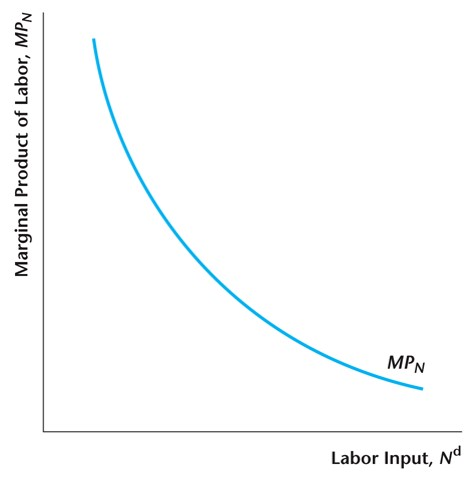
\includegraphics[width=\textwidth]{./figures/Figure4_14.jpg}
        \end{figure}
    \end{column}
    \begin{column}{0.5\textwidth}
        \begin{figure}
            \caption{Increasing Marginal Cross-product}
            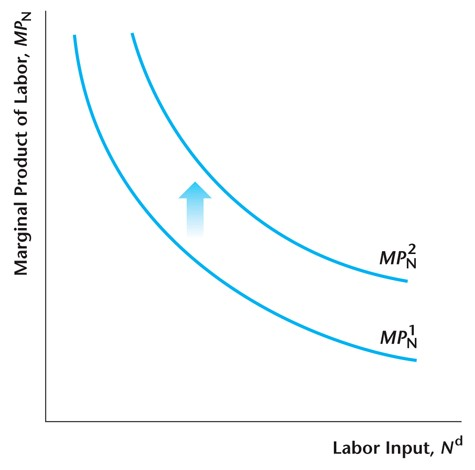
\includegraphics[width=\textwidth]{./figures/Figure4_15.jpg}
        \end{figure}
    \end{column}
\end{columns}
\end{frame}

\begin{frame}{Visualization: Changes in TFP}
\label{slide:Visualization__Changes_in_TFP}
\begin{columns}
    \begin{column}{0.5\textwidth}
        \begin{figure}
            \caption{TFP shifts up the Production Function}
            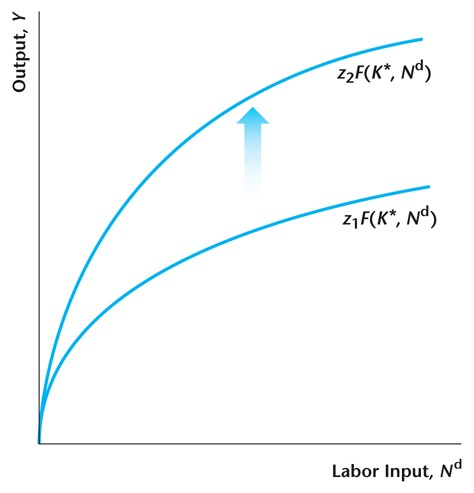
\includegraphics[width=\textwidth]{./figures/Figure4_16.jpg}
        \end{figure}
    \end{column}
    \begin{column}{0.5\textwidth}
        \begin{figure}
            \caption{TFP increases MPN}
            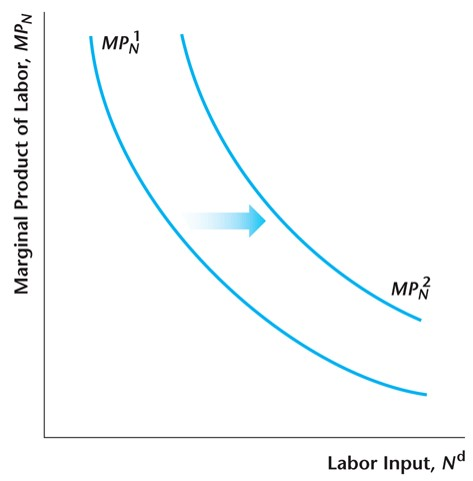
\includegraphics[width=\textwidth]{./figures/Figure4_17.jpg}
        \end{figure}
    \end{column}
\end{columns}

\end{frame}

\begin{frame}{TFP in Data}
\label{slide:TFP_in_Data}
    \begin{columns}
        \begin{column}{0.6\textwidth}
            \begin{figure}
                \caption{\alert{Solow Residual} for US}
                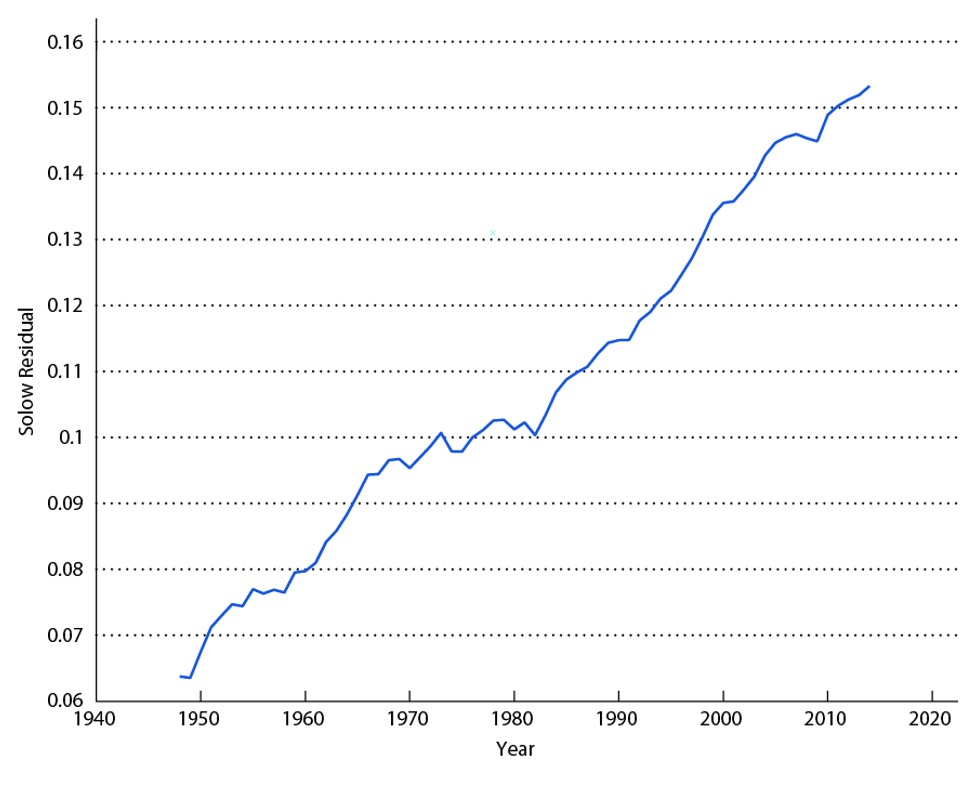
\includegraphics[width=\textwidth]{./figures/Figure4_18.jpg}
            \end{figure}
        \end{column}
        \begin{column}{0.4\textwidth}
            We cannot see TFP, \alert{how to measure it}?
            \begin{itemize}
                \item Assume Cobb-Douglas production function: $ Y = z K^{\alpha} N^{1-\alpha} $
                \item By data, $ K/Y = 0.3 $ $ \Rightarrow  $ $ \alpha = 0.3  $
                \item Can observe $ K $, $ Y $, $ N $ in data:
                %
                \begin{equation*}
                   z = \frac{Y}{K^{0.3}N^{0.7}}
                \end{equation*}
                %
            \end{itemize}
        \end{column}
    \end{columns}
\end{frame}

\section{Optimization}
\label{sec:Optimization}

\begin{frame}{Firm's Problem: Profit Maximization}
\label{slide:Firm_s_Problem__Profit_Maximization}
Firm maximizes profit ($\pi$), which is the revenue minus the wage bill:
\begin{equation}
\label{eq:profit}
    \pi = \max_{N^{d}} z F( K, N^{d} ) - w N^{d}
\end{equation}
\begin{itemize}
    \item \textbf{Constraints}: $ N^{d} > 0 $, relatively simple!
        %
        \begin{align}
            \text{Cobb-Douglas:} \quad
                & z F( K, N^{d} ) = z K^{\alpha} ( N^{d} )^{1-\alpha}
            \\
            \text{FOC:} \quad
                & w = z ( 1-\alpha ) K^{\alpha} ( N^{d} )^{-\alpha}
            \\
                & ( N^{d} )^{\alpha} = \frac{z ( 1-\alpha ) K^{\alpha}}{w}
            \\
            \text{Labor demand:} \quad
                & N^{d} = \left(
                    \frac{z ( 1-\alpha ) K^{\alpha}}{w}
                \right)^{\frac{1}{\alpha}}
                =
                \left(
                    \frac{z ( 1-\alpha ) }{w}
                \right)^{\frac{1}{\alpha}} K
        \end{align}
        %
        As $ w \uparrow  $, $ N^{d} \downarrow  $ $ \Rightarrow  $ \alert{downward-sloping} demand.
\end{itemize}
\end{frame}

\section{Experiments}
\label{sec:Experiments}

\begin{frame}{Experiment 1: Payroll Tax}
\label{slide:Experiment_1__Payroll_Tax}
    \textbf{Payroll tax:} suppose firms have to pay additional per-unit tax $ t > 0$ on the wage bill, then
    %
    \begin{align}
        \text{Firm Problem:} \quad
            & \max_{N^{d}} z K^{\alpha} ( N^{d} )^{1-\alpha} - w \red{( 1+\alert{t} )} N^{d}
        \\
        \text{FOC:} \quad
            & w( 1+t ) = z ( 1-\alpha ) K^{\alpha} ( N^{d} )^{-\alpha}
        \\
            & N^{d} = K \left(
                \frac{z ( 1-\alpha )}{w \red{( 1+t )}}
            \right)^{\frac{1}{\alpha}}
    \end{align}
    %
    \begin{itemize}
        \item \textbf{wage $ \uparrow  $}: $ w \uparrow  $ $ \Rightarrow  $ $ N^{d} \downarrow  $ (same as benchmark)
        \item \textbf{tax $ \uparrow  $}: $ t \uparrow  $ $ \Rightarrow  $ $ N^{d} \downarrow  $
        \item \textbf{capital $ \uparrow  $}: $ K \uparrow  $ $ \Rightarrow  $ $ N^{d} \uparrow  $ $ \Rightarrow  $ \alert{what if firm can also choose $ K $?}
    \end{itemize}
\end{frame}

\begin{frame}{Experiment 2: Choice of Capital}
\label{slide:Experiment_2__Choice_of_Capital}
    \textbf{Capital rent}: suppose that firm can choose capital level but have to pay $ r $ of per-unit rent.
    %
    \begin{align}
        \text{Firm Problem:} \quad
            & \max_{\red{K}, N^{d}} z K^{\alpha} ( N^{d} )^{1-\alpha} \red{- r K} - w N^{d}
        \\
        \text{FOC on N:} \quad
            & w = z ( 1-\alpha ) K^{\alpha} ( N^{d} )^{-\alpha}
            \label{eq:FOCN}
        \\
        \text{FOC on K:} \quad
            & r = z \alpha K^{\alpha-1} ( N^{d} )^{1-\alpha}
            \label{eq:FOCK}
        \\
        \text{Divide } \eqref{eq:FOCN} \text{ with } \eqref{eq:FOCK}: \quad
            & \frac{w}{r} = \frac{( 1-\alpha )}{\alpha} \frac{K}{N^{d}}
        \\
        \text{Capital-Labor ratio:} \quad
            & \frac{K}{N^{d}} = \frac{w}{r} \frac{\alpha}{1-\alpha}
            \label{eq:KLRatio}
    \end{align}
    %
    When firm can choose $ K $, they choose both capital and labor such that \eqref{eq:KLRatio} satisfied!
\end{frame}
\end{document}
